% ----- Compilar pdflatex -> pdflatex
\documentclass[12pt]{article}

\usepackage[utf8]{inputenc}
\usepackage[portuges]{babel}
\usepackage{multirow}
\usepackage{booktabs}
\usepackage[a4paper]{geometry}
\usepackage{amsmath}
\usepackage{graphicx}
\usepackage{float}
\usepackage{natbib}
\usepackage{hyperref} 
\usepackage{indentfirst}
\usepackage{xcolor}
\definecolor{dark-red}{rgb}{0.4,0.15,0.15}
\definecolor{dark-blue}{rgb}{0.15,0.15,0.5}
\definecolor{medium-blue}{rgb}{0,0,0.5}
\usepackage{listings}

\lstset{%
        inputencoding=utf8,
        extendedchars=true,
        literate=%
        {é}{{\'{e}}}1
        {è}{{\`{e}}}1
        {ê}{{\^{e}}}1
        {ë}{{\¨{e}}}1
        {É}{{\'{E}}}1
        {Ê}{{\^{E}}}1
        {û}{{\^{u}}}1
        {ù}{{\`{u}}}1
        {â}{{\^{a}}}1
        {à}{{\`{a}}}1
        {á}{{\'{a}}}1
        {ã}{{\~{a}}}1
        {Á}{{\'{A}}}1
        {Â}{{\^{A}}}1
        {Ã}{{\~{A}}}1
        {ç}{{\c{c}}}1
        {Ç}{{\c{C}}}1
        {õ}{{\~{o}}}1
        {ó}{{\'{o}}}1
        {ô}{{\^{o}}}1
        {Õ}{{\~{O}}}1
        {Ó}{{\'{O}}}1
        {Ô}{{\^{O}}}1
        {î}{{\^{i}}}1
        {Î}{{\^{I}}}1
        {í}{{\'{i}}}1
        {Í}{{\~{Í}}}1
}

\definecolor{mygreen}{rgb}{0,0.6,0}
\definecolor{mygray}{rgb}{0.5,0.5,0.5}
\definecolor{mymauve}{rgb}{0.58,0,0.82}

\lstset{ %
  backgroundcolor=\color{white},   % choose the background color; you must add \usepackage{color} or \usepackage{xcolor}
  basicstyle=\footnotesize,        % the size of the fonts that are used for the code
  breakatwhitespace=false,         % sets if automatic breaks should only happen at whitespace
  breaklines=true,                 % sets automatic line breaking
  captionpos=b,                    % sets the caption-position to bottom
  commentstyle=\color{mygreen},    % comment style
  deletekeywords={...},            % if you want to delete keywords from the given language
  escapeinside={\%*}{*)},          % if you want to add LaTeX within your code
  extendedchars=true,              % lets you use non-ASCII characters; for 8-bits encodings only, does not work with UTF-8
  frame=single,                    % adds a frame around the code
  keepspaces=true,                 % keeps spaces in text, useful for keeping indentation of code (possibly needs columns=flexible)
  keywordstyle=\color{blue},       % keyword style
  language=Octave,                 % the language of the code
  morekeywords={*,...},            % if you want to add more keywords to the set
  numbers=left,                    % where to put the line-numbers; possible values are (none, left, right)
  numbersep=5pt,                   % how far the line-numbers are from the code
  numberstyle=\tiny\color{mygray}, % the style that is used for the line-numbers
  rulecolor=\color{black},         % if not set, the frame-color may be changed on line-breaks within not-black text (e.g. comments (green here))
  showspaces=false,                % show spaces everywhere adding particular underscores; it overrides 'showstringspaces'
  showstringspaces=false,          % underline spaces within strings only
  showtabs=false,                  % show tabs within strings adding particular underscores
  stepnumber=2,                    % the step between two line-numbers. If it's 1, each line will be numbered
  stringstyle=\color{mymauve},     % string literal style
  tabsize=2,                       % sets default tabsize to 2 spaces
  title=\lstname                   % show the filename of files included with \lstinputlisting; also try caption instead of title
}

\hypersetup{
  colorlinks, linkcolor={dark-blue},
  citecolor={medium-blue}, urlcolor={dark-red}
}

% opening
\title{Distribuição Gamma}
\author{Bruno Normande}
\date{\today}

\begin{document}

\maketitle

\section{Introdução}

Esse trabalho faz uma análise do comportamento de três estimadores
para distribuição Gamma, quando estimados usando o método de Monte Carlo
comparando-os com suas versões usando \textit{bootstrap}.

Os estimadores usados nesse trabalho foram:

\begin{itemize}
  \item Estimador por máxima verossimilhança;
  \item Estimador pelo primeiro momento;
  \item Estimador pelo segundo momento central.
\end{itemize}

\section{Características da Distribuição Gamma}

A distribuíção Gamma é uma distribuíção que é caracterizda por dois
parâmentros, \textit{shape} ($k$) e \textit{scale} ($\theta$). Ela
possui a seguinte função densidade probabilidade:

\begin{align}
  f(w;k,\theta) & =
  \frac{w^{k-1}e^{\frac{w}{\theta}}}{\theta^k\Gamma(w)}
  \intertext{para}
  k,\theta > 0
\end{align}

Essa distribuição é usada muitas vezes para modelar o tempo de espera,
como por exemplo em teste de vida a distribuição Gamma é usada para
modelar o tempo até a morte. A figura \ref{fig:densidade} mostra o
comportamento de Gamma para diferentes valores de $k$ e $\theta$.

\begin{figure}[h!]
  \centering
  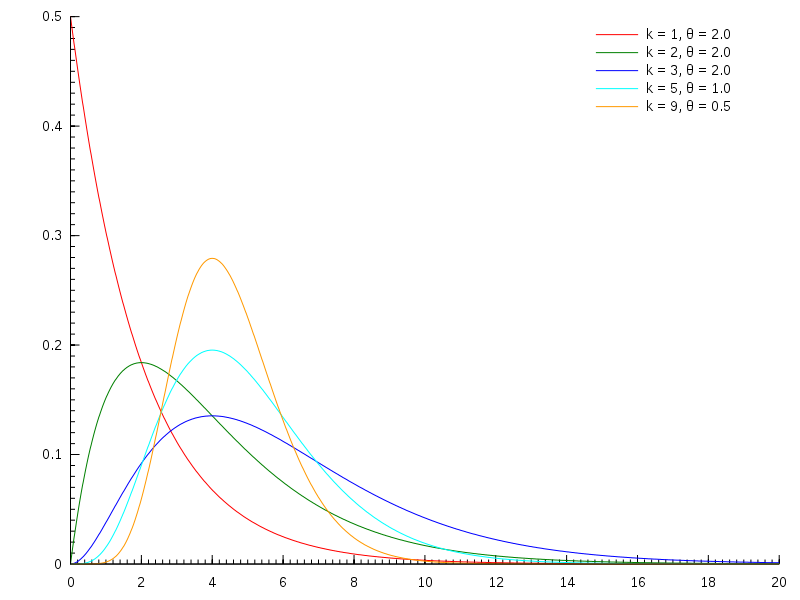
\includegraphics[width=.8\textwidth]{gamma_distribution.png}
  \caption{Função probabilidade Densidade de Gamma para diferentes parâmetros 
  				(imagem retirada de \url{http://en.wikipedia.org/wiki/Gamma_distribution})}
  \label{fig:densidade}
\end{figure}

Obtemos a esperança e a variância da distribuição com as seguintes
fórmulas:

\begin{align}
  E[W] &= k\theta\\
  Var[W] &= k\theta^2
\end{align}


\section{Estimadores}

Nesse trabalho foram analisados 6 estimadores para a distribuição
Gamma. Em todos foi usado $\theta = 1$ para manter a simplicidade dos
teste. Os estimadores usados foram:

\subsection{Estimador por Máxima Verossimilhança}

  Para estimar pela Máxima Verossimilhança é preciso maximizar a
  sua função log-verossimilhança de $\Gamma(w;k,1)$

  \small \begin{align}
            %    \label{eq:Gamma_MV}
    log(p(W|k,1)) &= n(k-1)\overline{log(x)} - n log(\Gamma(k)) - n k
    log(\overline{x}) +  n k log(a) - n k
    \intertext{Que podemos resolver numericamente iterando sobre k em:}
            %    log(p(W|k,1)) &\approx c_0 + c_1a + c_2log(a)
    \frac{1}{k_n} &= \frac{1}{k_{n-1}} + \frac{\overline{log(x)} -
      log(\overline{x}) + log(k_{n-1}) - \psi(k_{n-1})}{k_{n-1}^2 (\frac{1}{k_{n-1}} -
      \psi'(k_{n-1}))} \\
    \intertext{até o momento em que}
    k_n &\approx k_{n-1} \\
    \intertext{Como k inicial podemos usar a seguinte aproximação}
    \hat{k_0} &= \frac{0.5}{log(\overline{x}) - \overline{log(x)}}
  \end{align}
  
  Nesse trabalho usaremos a notação $\hat{k}_0$ para o estimador por máxima verossimilhança.

\subsection{Estimador pelo Primeiro Momento}

Usando o método dos momentos podemos estimar $k$ a partir do primeiro
momento da seguinte maneira:

\begin{align}
  % \label{eq:G_m_p2}
  E[W] &= k\theta \\
  \hat{k} &= \frac{1}{n} \sum_{i=1}^nw_i 
\end{align}

  Nesse trabalho usaremos a notação $\hat{k}_1$ para o estimador pelo primeiro momento.

\subsection{Estimador pelo Segundo Momento Central}

De maneira similar podemos estimar $k$ a partir do segundo
momento central da seguinte maneira:

\begin{align}
  % \label{eq:G_m_p3}
  Var[W] &= k\theta^2 \\
  \hat{k} &= Var(w) 
\end{align}

  Nesse trabalho usaremos a notação $\hat{k}_2$ para o estimador pelo segundo momento central.

\subsection{Estimadores com \textit{bootstrap}}

Todos os estimadores mencionados àcima foram testados também contra
suas versões com \textit{bootstrap}. Dessa maneira foi possível
observar se usando o método \textit{bootstrap} poderiamos diminuir o
viés desses estimadores.

Como notação para identificar estes estimadores foi usado um til no
lugar do chápeu:

\begin{align*}
  \tilde{k}_0, \tilde{k}_1\ e\ \tilde{k}_1^2
\end{align*}

% Sua esperança é $1/\lambda$ e sua variância $1/\lambda^2$.

% Os momentos se dão pela fórmula $n!/\lambda^n$, (n = 1, 2, 3 ...). Assim, seu primeiro momento é igual a sua esperança $(1/\lambda)$ e seu segundo momento se dá por $2/\lambda^2$. Seus estimadores são, respectivamente, $\sqrt{1/var(x)}$ e $\sqrt{1/mean^2}$. 

% A máximo verossimilhança é dada por $1/\bar{x}$.


\section{Resultados}

As tabelas a seguir comparam os estimadores usados com suas versões
\textit{bootstraped}. 

\begin{table}[H]
  
  \label{tab:gamma_r_mv}
  \centering
  \begin{tabular}{rccc}
    \toprule
    \multicolumn{4}{c}{Comparação dos Estimadores $\hat{k}$ e $\tilde{k}$}\\
    $n$ & $k$ & $|B(\hat{k})|>|B(\tilde{k})|$ & $EQM(\hat{k})>EQM(\tilde{k})$ \\
    \midrule
    100 & 1 & TRUE & TRUE\\
    1000 & 1 & FALSE & FALSE\\
    10000 & 1 & FALSE & TRUE\\
    100000 & 1 & FALSE & FALSE\\
    100 & 2 & TRUE & TRUE\\
    1000 & 2 & TRUE & FALSE\\
    10000 & 2 & FALSE & FALSE\\
    100000 & 2 & FALSE & FALSE\\
    100 & 3 & TRUE & TRUE\\
    1000 & 3 & FALSE & FALSE\\
    10000 & 3 & FALSE & FALSE\\
    100000 & 3 & TRUE & FALSE\\
    100 & 5 & TRUE & TRUE\\
    1000 & 5 & FALSE & FALSE\\
    10000 & 5 & FALSE & TRUE\\
    100000 & 5 & FALSE & TRUE\\
    100 & 9 & FALSE & TRUE\\
    1000 & 9 & TRUE & TRUE\\
    10000 & 9 & FALSE & FALSE\\
    100000 & 9 & TRUE & TRUE\\
    \bottomrule
  \end{tabular}
  \caption{Estimadores de máxima verossimilhança $\hat{k}$ e $\tilde{k}$.}
\end{table}

\begin{table}[H]
  \label{tab:gamma_r_m1}
  \centering
  \begin{tabular}{rccc}
    \toprule
    \multicolumn{4}{c}{Comparação dos Estimadores $\hat{k}_1$ e $\tilde{k}_1$}\\
    $n$ & $k$ & $|B(\hat{k}_1)|>|B(\tilde{k_1})|$ & $EQM(\hat{k}_1)>EQM(\tilde{k}_1)$ \\
    \midrule
    100 & 1 & FALSE & FALSE\\
    1000 & 1 & FALSE & FALSE\\
    10000 & 1 & TRUE & FALSE\\
    100000 & 1 & FALSE & FALSE\\
    100 & 2 & FALSE & FALSE\\
    1000 & 2 & TRUE & FALSE\\
    10000 & 2 & FALSE & FALSE\\
    100000 & 2 & FALSE & FALSE\\
    100 & 3 & FALSE & FALSE\\
    1000 & 3 & FALSE & FALSE\\
    10000 & 3 & FALSE & FALSE\\
    100000 & 3 & FALSE & FALSE\\
    100 & 5 & FALSE & FALSE\\
    1000 & 5 & FALSE & FALSE\\
    10000 & 5 & FALSE & FALSE\\
    100000 & 5 & FALSE & FALSE\\
    100 & 9 & FALSE & FALSE\\
    1000 & 9 & FALSE & FALSE\\
    10000 & 9 & TRUE & FALSE\\
    100000 & 9 & FALSE & FALSE\\
    \bottomrule
  \end{tabular}
  \caption{Estimadores de primeiro momento $\hat{k}_1$ e $\tilde{k}_1$.}
\end{table}

\begin{table}[H]
  \label{tab:gamma_r_m1}
  \centering
  \begin{tabular}{rccc}
    \toprule
    \multicolumn{4}{c}{Comparação dos Estimadores $\hat{k}_2^0$ e $\tilde{k}_2^0$}\\
    $n$ & $k$ & $|B(\hat{k}_2^0)|>|B(\tilde{k_2^0})|$ & $EQM(\hat{k}_2^0)>EQM(\tilde{k}_2^0)$ \\
    \midrule
    100 & 1 & FALSE & FALSE\\
    1000 & 1 & TRUE & FALSE\\
    10000 & 1 & FALSE & FALSE\\
    100000 & 1 & FALSE & FALSE\\
    100 & 2 & FALSE & FALSE\\
    1000 & 2 & TRUE & FALSE\\
    10000 & 2 & FALSE & FALSE\\
    100000 & 2 & FALSE & FALSE\\
    100 & 3 & FALSE & FALSE\\
    1000 & 3 & TRUE & FALSE\\
    10000 & 3 & FALSE & FALSE\\
    100000 & 3 & FALSE & FALSE\\
    100 & 5 & FALSE & FALSE\\
    1000 & 5 & FALSE & FALSE\\
    10000 & 5 & FALSE & FALSE\\
    100000 & 5 & FALSE & FALSE\\
    100 & 9 & TRUE & FALSE\\
    1000 & 9 & FALSE & FALSE\\
    10000 & 9 & TRUE & FALSE\\
    100000 & 9 & FALSE & FALSE\\
    \bottomrule
  \end{tabular}
  \caption{Estimadores de segundo momento central $\hat{k}_2^0$ e $\tilde{k}_2^0$.}
\end{table}

\section{Conclusão}

Analisando os resultados podemos ver que para a distribuição Gamma
o método \textit{bootstrap} não melhorou o viés dos estimadores o que
nos leva à conclusão de que esse método não deve ser usado para essa
distribuição.

Para confirmar essa conclusão futuros estudos devem ser feitos usando essa
distribuição e mais valores de $n$ e $k$.

\newpage
\appendix
\section{Código em R Usados no Trabalho}

Estimadores.

\lstinputlisting{gamma_estimators.R}

Script de teste.

\lstinputlisting{ensaio_montecarlo.R}

\end{document}



